\section{Задание 4. Системы ДУ. Устойчивость.}

\textbf{Условие.}

Дана система ДУ:

\[\begin{cases}\frac{dx}{dt} = -2x + 5y, \\ \frac{dy}{dt} = 2x + y\end{cases}\]

\begin{enumerate}
    \item Найдите общее решение системы.
    \item Изобразите на фазовой плоскости семейство интегральных кривых $y = y(x)$.
    \item Исследуйте решение системы на устойчивость при $t \to +\infty$.
    \item Определите характер особой точки.
\end{enumerate}

\vspace{10mm}
\textbf{Решение.}

\begin{enumerate}
    \item решение ДУ
    
    Решим через метод Эйлера (через характерестическое уравнение).

    В общем наше решение будет выглядеть как система функций вида:

    \begin{equation*}
        \begin{cases}
          x(t) = \omega_1 C_1 e^{\lambda_1t} + \omega_2 C_2 e^{\lambda_1t}
          \\
          y(t) = \mu_1 C_1 e^{\lambda_2t} + \mu_2 C_2 e^{\lambda_2t}
        \end{cases}
       \end{equation*}
         

    $\displaystyle \begin{bmatrix}
        -2 && 5 \\
        2 && 1 \\
   \end{bmatrix} = $
   $\displaystyle \begin{bmatrix}
       -2 - \lambda && 5 \\
       2 && 1 - \lambda \\
  \end{bmatrix} $

  $(-2-\lambda)(1-\lambda) - 2*5 = 0$
  $\Rightarrow \lambda^2 + \lambda - 12 = 0$
  $\Rightarrow \lambda_{1,2} = -4, 3$

  \begin{multicols}{2}
    \begin{subtasks}
        \item $\lambda_1 = -4$
        $\displaystyle \begin{bmatrix}
            2 && 5 \\
            2 && 5 \\
       \end{bmatrix} \Rightarrow \omega_1 = -\frac{5}{2} \mu_1 $ \\ (возьмем $\mu_2 = 1$, тогда $\omega_1 = -\frac{5}{2}$). 
        \item $\lambda_2 = 3$
        $\displaystyle \begin{bmatrix}
            -5 && 5 \\
            2 && -2 \\
       \end{bmatrix} \Rightarrow \omega_2 = \mu_2 $ \\ (возьмем любое число, к примеру: 1).
    \end{subtasks}
    \end{multicols}

    Тогда наша система выглядит так:

    \begin{equation*}
     \begin{cases}
       x(t) = -\frac{5}{2} C_1 e^{-4t} + C_2 e^{3t}
       \\
       y(t) = C_1 e^{-4t} + C_2 e^{3t}
     \end{cases}
    \end{equation*}
      

    \item Фазовая плоскость

    Т.к. собственные числа характерестического уравнения действительные и разных знаков то фазовая плоскость будет состоять
     как бы из гипербол. Поэтому нам нужно найти векторы асимптот. Каждый такой вектор $x_i$ можно найти через уравнение
     $\displaystyle \begin{bmatrix}
        -2 - \lambda_i && 5 \\
        2 && 1 - \lambda_i \\
   \end{bmatrix} * x_i = 
   \begin{bmatrix}
    0 \\
    0 \\
\end{bmatrix} 
   $

   Таким образом: $
   x_1 = 
   \begin{bmatrix}
    5 \\
    -2 \\
\end{bmatrix} ,
x_2 = 
\begin{bmatrix}
    -1 \\
    -1 \\
\end{bmatrix} 
   $

   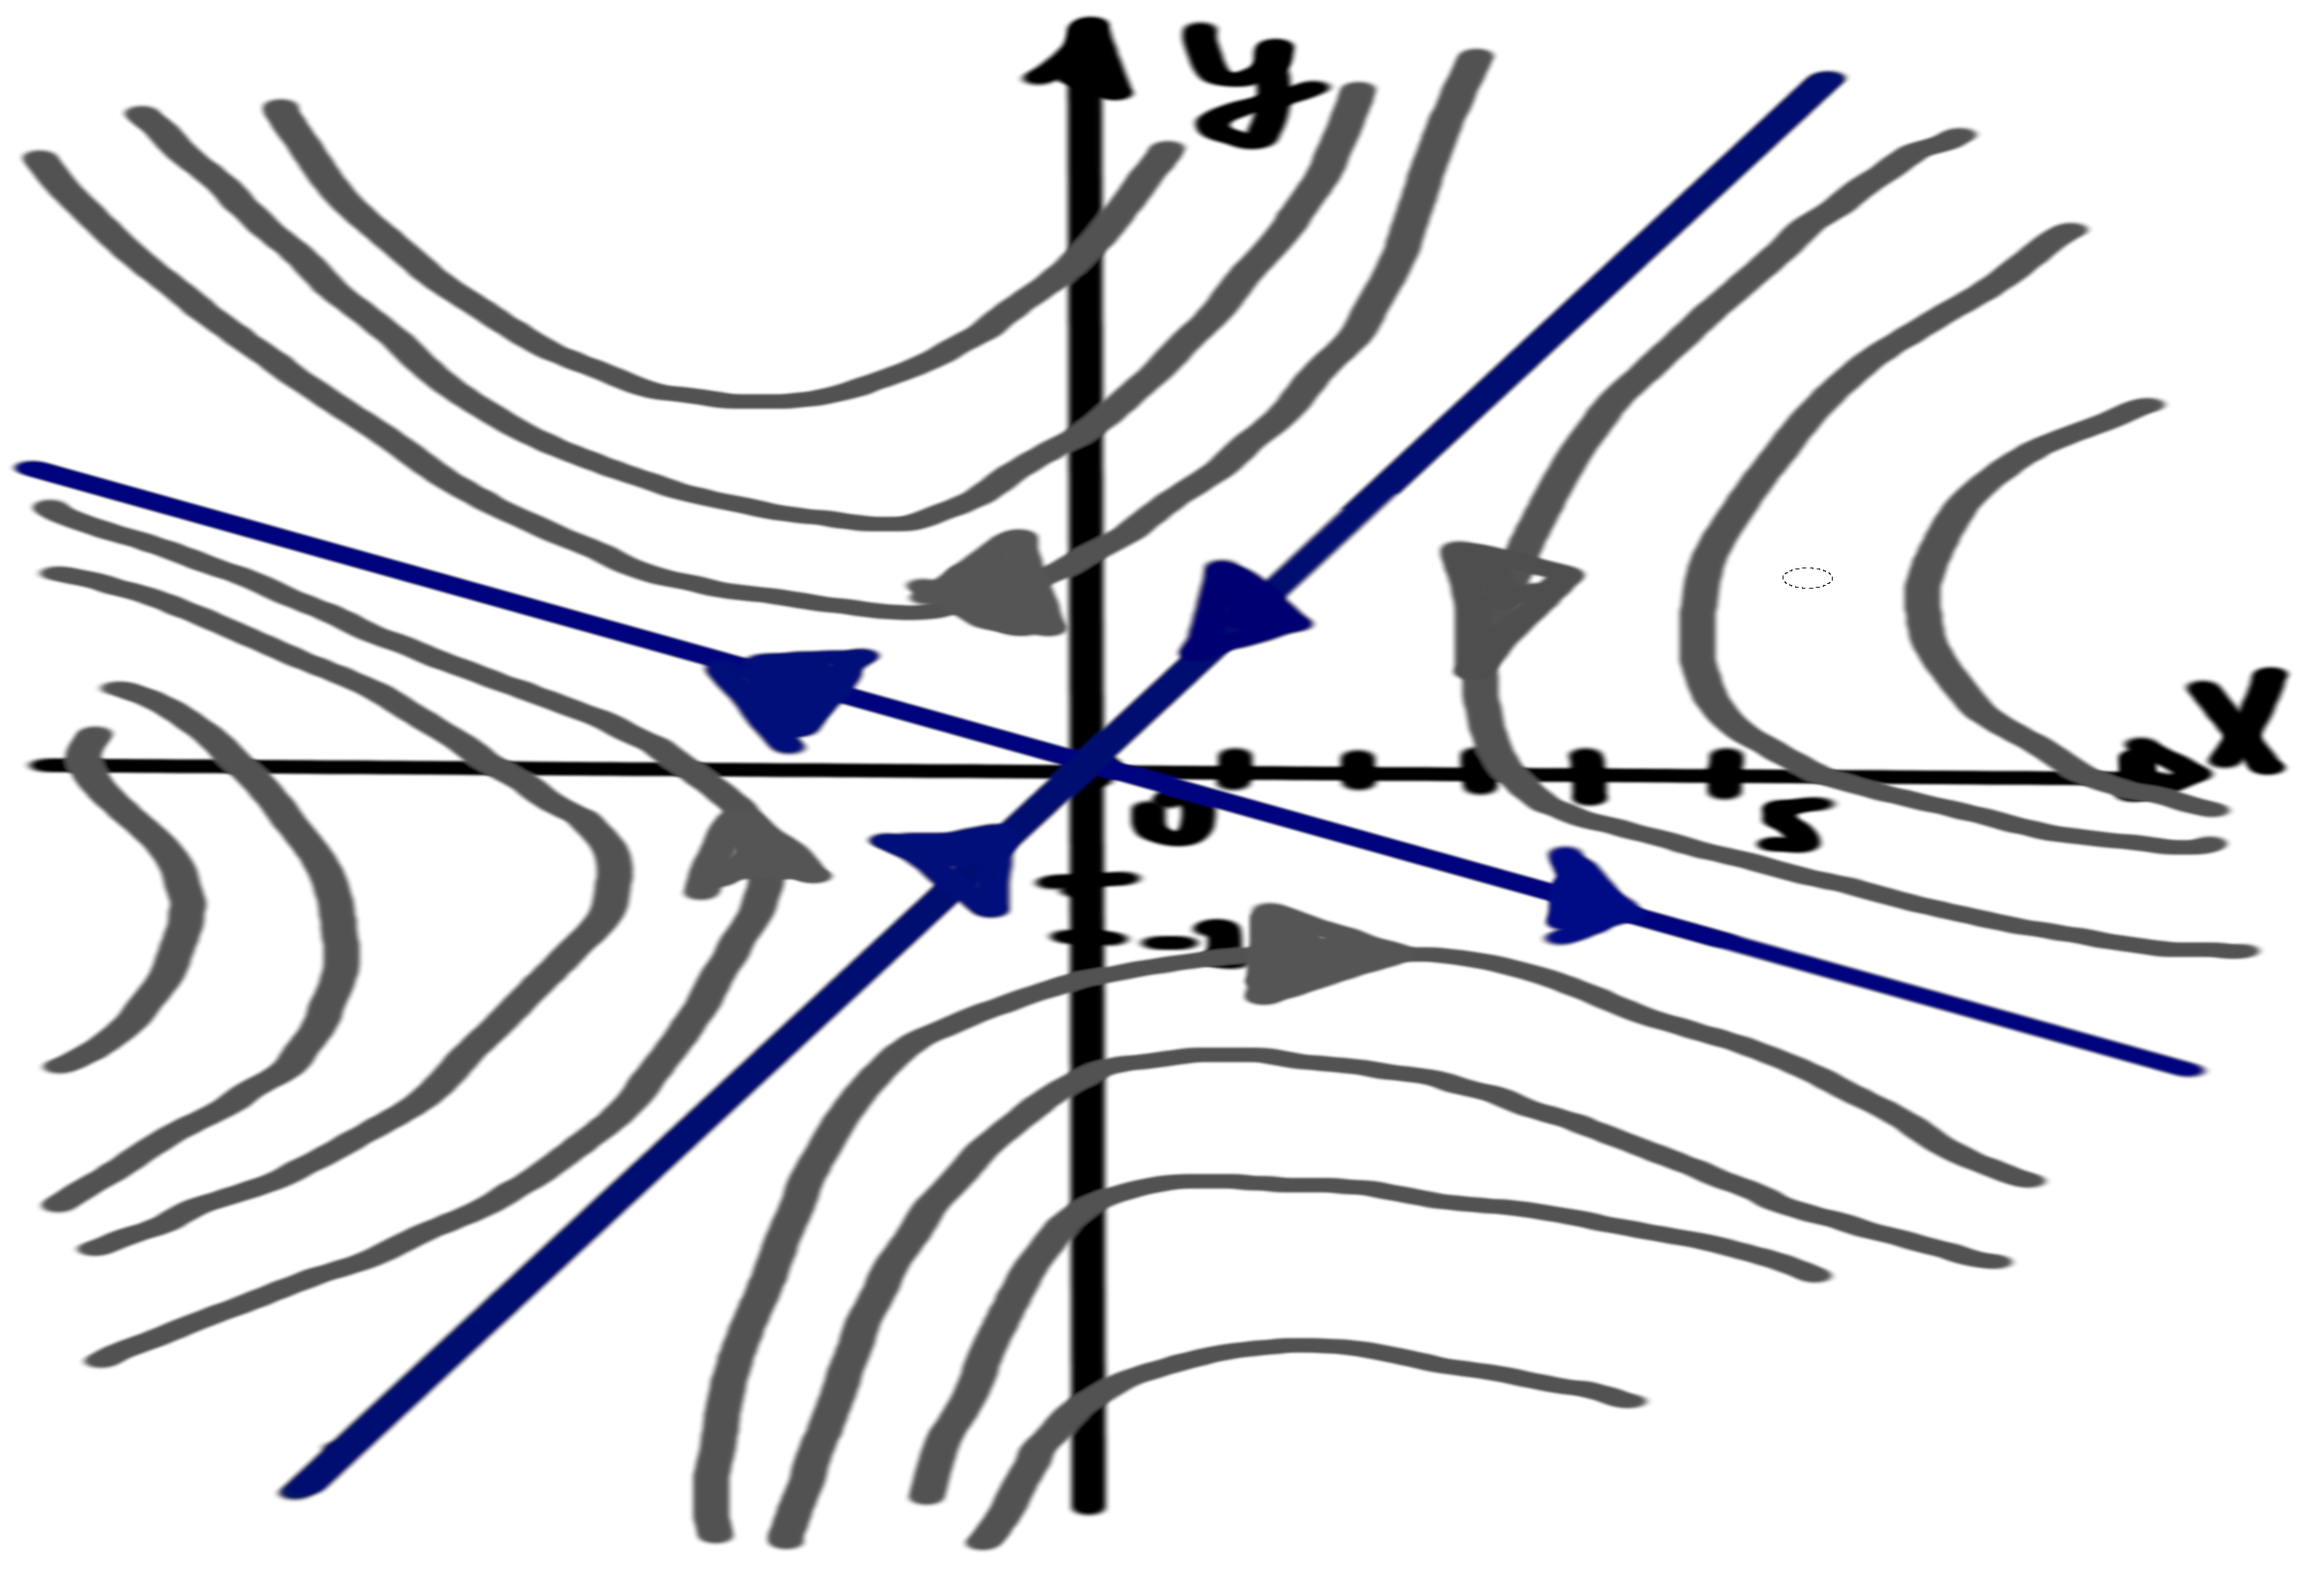
\includegraphics[scale=0.2]{ss34task.png}

    \item Устойчивость: Т.к. корни характерестического уравнения действительные числа одного знака, то
    положение равновесия которое у нас получится - седло.
    \item Тип особоый точки: (0, 0) - седло
\end{enumerate}

